\documentclass{article}
\usepackage{listings}
\usepackage{graphicx} % Required for inserting images
\graphicspath{ {https://www.overleaf.com/project/6478a2664987ff17798908a3/file/6481e9c10997cddc341788e7} }
\graphicspath{https://www.overleaf.com/project/6478a2664987ff17798908a3/file/64845ab4451af1fa32f76d9b}
\graphicspath{https://www.overleaf.com/project/6478a2664987ff17798908a3/file/6486ad6a47ddd5e42fea197f}
\usepackage[a4paper, total={6in, 8in}]{geometry}

\begin{document}
\begin{center}
\begin{figure}
\centering

\includegraphics[scale = 0.35]{image.png}\\
The AI-ML and Data Science Club of IITH
\end{figure}
\end{center}

\begin{center}
    {\LARGE{\textbf{Algorithms to Solve Multi-Arm Bandit Problem-I}}}
\end{center}


\graphicspath{{./media/}}
\begin{center}
    \large{\textbf{{Contents}}}
\end{center}



\begin{enumerate}
 \item {Multi-Arm Bandit: Setting}\\
 \item {Multi-Arm Bandit: Formulation}\\
 \item {Regret Minimization}\\
 \item {Regret Minimization: Alternative Formulation}\\
 \item {Linear and Sub-Linear Regret}\\
 \item {Naive Approaches}\\
 \indent{6.1 Greedy Algorithm}\\
 \indent{6.2 Explore then Commit Algorithm}
\end{enumerate}

\begin{center}
    {\textbf{Compiled by :}
    \texttt{Sriram Gonella}
\end{center}

\newpage
\section{Multi-Arm Bandit: Setting}
First, we will try to establish the bandit setting. Let us consider a multi-arm bandit with $\textbf{K}$ arms, and you are provided with $\textbf{N}$ rounds. You are allowed to pull any of the $\textbf{K}$ arms in each round $\textbf{t $\in$ {1, 2, 3, 4....., N}}$. On pulling arm $a$, the agent gets a random reward $\textbf{$r_{a}$}$ sampled from a distribution(independent of previous choices and rewards). The goal is to find an algorithm that maximizes the sum of rewards obtained by pulling
arm (in expectation).
\section{Multi-Arm Bandit: Formulation}
A multi-arm bandit can be defined as a tuple $<A, R>$. $<A>$ is the set of arms available. $R^a(r)=P(r|a)$ is the unknown distribution of rewards of arm $a$. At each step $t$, the agent selects an action $a_t \in A$ and gets a reward $r_t $~$ R^{a_t}$. The goal is to maximize cumulative reward $\Sigma_{t=1}^{N} r_t$.
\section{Regret Minimization}
The goal is to maximize cumulative reward $\Sigma_{t=1}^{N} r_t$. Define the action value function $Q(a)$ to be the mean reward for action $a$ i.e. $Q(a) = E(r|a)$. The optimal value of $V^{*}$ is
\begin{equation} \label{eu_eqn}
V^* = Q(a^*) = \max_{a \in A} Q(a)
\end{equation}
The regret is the lost opportunity at one step
\begin{equation} \label{eu_eqn}
l_{t}=E[V^{*}-r_{t}]=V^{*}-E[r_{t}]
\end{equation}
Total regret is the total opportunity loss
\begin{equation} \label{eu_eqn}
L_{N}=E[\sum_{t=1}^{N}(V^{*}-r_{t})]=NV^{*}-E[\sum_{t=1}^{N}r_{t}]
\end{equation}
So to achieve maximum cumulative reward, the total regret must be minimized.
\section{Regret Minimization: Alternative Formulation}
Let the $\textbf{count} N_{t}(a)$ be the number of times arm $a$ is pulled up to time $t$. ($N_{t}(a)\equiv\sum_{T=1}^{t}1_{A_{T}=a}$). Let $\Delta_{a}$ be the gap between the optimal reward (from optimal action $a^{*}$) and the reward of the arm $a$
\begin{equation} \label{eu_eqn}
\Delta_{a}=V^{*}-Q(a)
\end{equation}
Regret is the function of gaps and counts given as
\begin{equation} \label{eu_eqn}
L_{N}=E[\sum_{t=1}^{N}(V^{*}-r_{t})]=E[\sum_{t=1}^{N}\Delta_{A_{t}}]=E[\sum_{t=1}^{N}\sum_{T=1}^{t}1_{A_{T}=a}\Delta_{a}]=\sum_{a \in A}\Delta_{a}E[N_{N}(a)]
\end{equation}
A good algorithm ensures small counts for large gaps.
\section{Linear and Sub-Linear Regret}
\begin{center}
    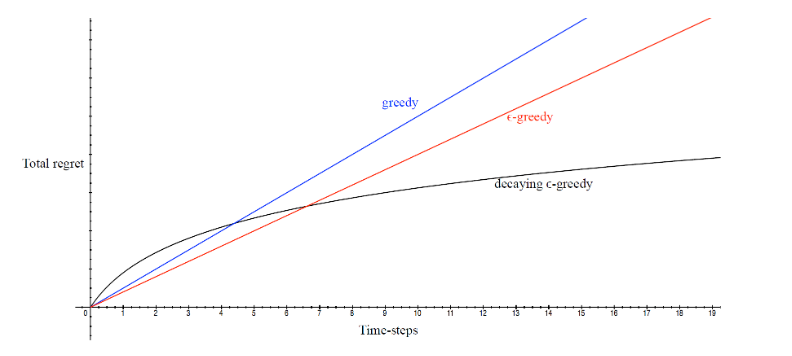
\includegraphics{pic1.png}
\end{center}

$\Rightarrow$ $\textbf{Algorithms that explore forever have total linear regret}.$ 
Let's consider an algorithm that explores forever. This means that the algorithm will always choose a random action with some probability, even if it has already learned that a different action is more optimal. In other words, the algorithm will never be 100\% certain about which action to take.
This has the following consequences:

\begin{enumerate}
    \item The algorithm will never achieve a perfect score. Even if the algorithm has learned the optimal policy, it will still make mistakes due to exploration.
    \item The algorithm's regret will grow linearly with time. This is because the algorithm will continue to make mistakes, and each mistake will add to its regret.
\end{enumerate}

To prove this, let's consider a simple example. Suppose there are two actions, $A$ and $B$, and the optimal policy is to always choose action $A$. Let's also suppose that the algorithm explores with probability $\epsilon$.

The expected regret of the algorithm after the $T$ steps is then given by:
\begin{equation} \label{eu_eqn}
E[R_{T}]\equiv T \times \epsilon \times (R_{A}-R_{B})
\end{equation}


where $R_A$ is the reward for action $A$ and $R_B$ is the reward for action $B$. We can see that the expected regret is linear in $T$. This is because the algorithm will explore with probability $\epsilon$ on each step, and each exploration will add to its regret. This result holds for any algorithm that explores forever. In other words, any algorithm that explores forever will have total linear regret.

$\Rightarrow$ $\textbf{Algorithms that never explore have total linear regret.}$  Let's consider an algorithm that never explores. This means that the algorithm will always choose the same action, even if it is not the optimal action. In other words, the algorithm will never learn from its mistakes.

This has the following consequences:
\begin{enumerate}
    \item The algorithm will never achieve a perfect score. Even if the algorithm starts with the optimal action, it will never learn to adapt to changes in the environment.
    \item The algorithm's regret will grow linearly with time. This is because the algorithm will continue to make the same mistake, and each mistake will add to its regret.
\end{enumerate}
As considered above. Suppose there are two actions, $A$ and $B$, and the optimal policy is to always choose action $A$. Let's also suppose that the algorithm always chooses action $B$.

The expected regret of the algorithm after $T$ steps is then given by:
\begin{equation} \label{eu_eqn}
E[R_{T}]\equiv T \times (R_{A}-R_{B})
\end{equation}
We can see that the expected regret is linear in $T$. This is because the algorithm will always choose action $B$, which is suboptimal, and each choice of action $B$ will add to its regret.

This result holds for any algorithm that never explores. In other words, any algorithm that never explores will have total linear regret.

Now let us look into the actual algorithms and their pseudo codes to solve a multi-arm bandit problem.

\section{Naive Approaches}
\subsection{Greedy Algorithm}
At any time $t$, a greedy algorithm selects the action with the highest $\hat{Q}_{t}(a)$, i.e.
\begin{equation} \label{eu_eqn}
a_{t}^{*} \equiv arg\max_{a \in A} \hat{Q}_{t}(a)
\end{equation}
The greedy algorithm can lock into a sub-optimal arm forever. We have discussed earlier that the greedy algorithm has total linear regret. The agent always selects the arm that is estimated to have the highest reward at any given time step. It prioritizes the exploitation of the currently perceived best arm without any exploration, leading to potential limitations in finding the truly optimal arm.

To understand how the completely greedy algorithm works, let's consider an example scenario. Suppose you have three slot machines in a casino, labeled $A, B, and C$. Each machine has an unknown probability distribution of winning, and your goal is to maximize your total winnings over a certain number of rounds.

Initially, since you have no information about the machines, you randomly select one of the arms to start. Let's say you choose to arm $A$ and receive a reward of $5$. Based on this single data point, you estimate that arm $A$ has the highest reward among the three arms.

Now, using the completely greedy algorithm, you always select arm A in subsequent rounds because it is currently perceived as the best arm. Let's say you play arm $A$ for the next 10 rounds and receive rewards of $3, 4, 2, 5, 3, 4, 2, 4, 3, and 2$. The average reward of arms A based on these rounds is $(3+4+2+5+3+4+2+4+3+2)/10 = 3.2$.

However, during these 10 rounds, you didn't explore other arms like $B and C$. It is possible that one of these unexplored arms could have a higher average reward than arm $A$. For instance, arm $B$ might have an average reward of $4.5$, and arm $C$ might have an average reward of $3.8$. But because the completely greedy algorithm only exploits the perceived best arm, it misses the opportunity to discover higher-rewarding arms.

In this example, the completely greedy algorithm suffers from a limitation known as "exploitation-only" or "greedy myopia." It prioritizes exploitation without any exploration, leading to potentially suboptimal decisions. The algorithm's estimate of the best arm can be inaccurate or biased due to a limited number of samples.

The implementation of this algorithm in Python is as follows:

\begin{lstlisting}[language = Python]
    
import numpy as np

class BanditArm:
    def __init__(self, true_reward):
        self.true_reward = true_reward
        self.estimated_reward = 0
        self.num_pulls = 0

    def pull(self):
        # Simulate pulling the arm and getting a reward (in this case, randomly generated)
        reward = np.random.normal(self.true_reward, 1)
        self.update_estimated_reward(reward)
        self.num_pulls += 1
        return reward

    def update_estimated_reward(self, reward):
        # Update the estimated reward using incremental averaging
        self.estimated_reward = (
            ((self.num_pulls - 1) * self.estimated_reward) + reward
        ) / self.num_pulls if self.num_pulls > 0 else reward

class GreedyAgent:
    def __init__(self, bandit_arms):
        self.bandit_arms = bandit_arms

    def choose_arm(self):
        # Select the arm with the highest estimated reward
        return max(self.bandit_arms, key=lambda arm: arm.estimated_reward)

    def play_round(self):
        chosen_arm = self.choose_arm()
        reward = chosen_arm.pull()
        return reward

# Define the number of arms and their true rewards
num_arms = 3
true_rewards = [3, 4, 5]

# Create the bandit arms
bandit_arms = [BanditArm(reward) for reward in true_rewards]

# Create the greedy agent
agent = GreedyAgent(bandit_arms)

# Run the simulation for a specified number of rounds
num_rounds = 1000
total_reward = 0

for _ in range(num_rounds):
    reward = agent.play_round()
    total_reward += reward

# Calculate the average reward
average_reward = total_reward / num_rounds

print("Average reward:", average_reward)
\end{lstlisting}

\begin{enumerate}
    \item The \textbf{BanditArm} class represents an arm of the bandit problem. It initializes with a true reward, estimated reward, and the number of times it has been pulled. The \textbf{pull} method simulates pulling the arm and updates the estimated reward using incremental averaging.
    
    \item The \textbf{GreedyAgent} class represents the agent that follows the completely greedy algorithm. It takes a list of the bandit's arms as input and has a \textbf{choose\_arm} method that selects the arm with the highest estimated reward. The \textbf{play\_round} method chooses an arm, pulls it, and returns the reward.

    \item In the main part of the code, you define the number of arms and their true rewards. Then, you create the bandit arms using the \textbf{BanditArm} class and the greedy agent using the \textbf{GreedyAgent} class.

    \item The simulation runs for a specified number of rounds, and in each round, the agent plays a round using the \textbf{play\_round} method. The total reward is accumulated.

    \item Finally, the average reward per round is calculated and printed.
\end{enumerate}


\subsection{Explore then Commit Algorithm}
 "Explore then Commit"  combines exploration and exploitation in two distinct phases. It begins with an initial exploration phase where the algorithm gathers information about the arms, followed by a commitment phase where it commits to exploiting the best arm based on the gathered information.

Let's illustrate the "Explore then Commit" algorithm with an example. Suppose you have four slot machines in a casino labeled $A, B, C, and D$. Your objective is to maximize your total winnings over a fixed number of rounds.
\begin{enumerate}
\item \textbf{Explore Phase:}
In the initial exploration phase, the algorithm randomly selects arms and collects data about their rewards. It allocates a certain number of rounds for exploration. Let's say we allocate $20$ rounds for exploration.

During the exploration phase, the algorithm randomly selects arms in a round-robin fashion. It plays each arm an equal number of times to gather information about their rewards. For example, it may play each arm five times during the exploration phase.

\item \textbf{Gather Information:}
As the algorithm plays each arm multiple times, it keeps track of the rewards obtained from each arm. It calculates the average reward for each arm based on the collected data.

\item \textbf{Identify the Best Arm:}
After the exploration phase, the algorithm determines which arm has the highest average reward based on the gathered information. Let's say it determines that arm $C$ has the highest average reward among the four arms.

\item \textbf{Commit Phase:}
In the commitment phase, the algorithm solely focuses on exploiting the arm that was identified as the best during the exploration phase. It allocates the remaining rounds, after the exploration phase, to fully exploit the identified best arm.
\end{enumerate}
During the commitment phase, the algorithm plays the best arm exclusively without any further exploration. It aims to maximize its rewards by exploiting the arm it believes to be the most rewarding based on the gathered information during the exploration phase.

The "Explore then Commit" algorithm strikes a balance between gathering information through exploration and maximizing rewards through exploitation. It combines the advantages of exploration to avoid prematurely committing to suboptimal arms with the benefits of exploitation to fully exploit the identified best arm.

It's worth noting that the success of the "Explore then Commit" algorithm depends on the accuracy of the information gathered during the exploration phase. If the exploration phase does not allocate enough rounds or fails to sufficiently explore the arms, the algorithm may not identify the true best arm, leading to suboptimal results during the commitment phase. Careful consideration should be given to the allocation of rounds for exploration to ensure reliable estimates of arm rewards.
Now let's see the pseudo-code for this algorithm

\begin{center}
    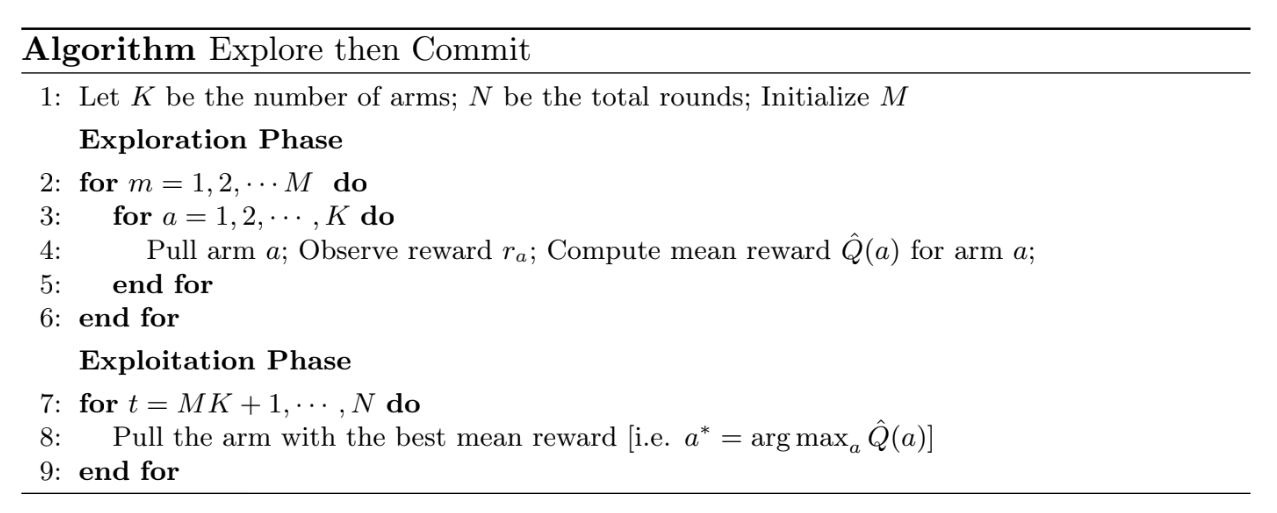
\includegraphics[scale = 0.55]{pic2.png}    
\end{center}

\begin{lstlisting}
import numpy as np

class BanditArm:
    def __init__(self, true_reward):
        self.true_reward = true_reward
        self.estimated_reward = 0
        self.num_pulls = 0

    def pull(self):
        # Simulate pulling the arm and getting a reward (in this case, randomly generated)
        reward = np.random.normal(self.true_reward, 1)
        self.update_estimated_reward(reward)
        self.num_pulls += 1
        return reward

    def update_estimated_reward(self, reward):
        # Update the estimated reward using incremental averaging
        self.estimated_reward = (
            ((self.num_pulls - 1) * self.estimated_reward) + reward
        ) / self.num_pulls if self.num_pulls > 0 else reward

class ExploreThenCommitAgent:
    def __init__(self, bandit_arms, exploration_rounds):
        self.bandit_arms = bandit_arms
        self.exploration_rounds = exploration_rounds
        self.best_arm = None
        self.rounds_played = 0

    def explore_phase(self):
        for _ in range(self.exploration_rounds):
            for arm in self.bandit_arms:
                arm.pull()

    def commit_phase(self):
        self.best_arm = max(self.bandit_arms, key=lambda arm: arm.estimated_reward)

    def choose_arm(self):
        if self.rounds_played < self.exploration_rounds:
            return self.bandit_arms[self.rounds_played % len(self.bandit_arms)]
        else:
            return self.best_arm

    def play_round(self):
        chosen_arm = self.choose_arm()
        reward = chosen_arm.pull()
        self.rounds_played += 1
        return reward

# Define the number of arms and their true rewards
num_arms = 4
true_rewards = [3, 4, 5, 2]

# Create the bandit arms
bandit_arms = [BanditArm(reward) for reward in true_rewards]

# Create the Explore then Commit agent with an exploration phase of 20 rounds
exploration_rounds = 20
agent = ExploreThenCommitAgent(bandit_arms, exploration_rounds)

# Explore phase
agent.explore_phase()

# Commit phase
agent.commit_phase()

# Run the simulation for a specified number of rounds after exploration
num_rounds_after_exploration = 1000
total_reward = 0

for _ in range(num_rounds_after_exploration):
    reward = agent.play_round()
    total_reward += reward

# Calculate the average reward
average_reward = total_reward / num_rounds_after_exploration

print("Average reward:", average_reward)

\end{lstlisting}
    


The above code snippets give the implementation of the Explore and then Commit algorithm in Python.

\begin{enumerate}
    \item The \textbf{BanditArm} class is the same as before, representing an arm of the bandit problem with true rewards and estimated rewards.

    \item The \textbf{ExploreThenCommitAgent} class is specifically designed for the "Explore then Commit" algorithm. It takes the bandit arms and the number of rounds to allocate for exploration as input.

    \item The agent has an \textbf{explore\_phase} method that randomly selects arms and pulls them to gather information during the exploration phase.

    \item After the exploration phase, the agent has a \textbf{commit\_phase} method that identifies the best arm based on the gathered information.

    \item The \textbf{choose\_arm} method selects the arm for each round. If the number of rounds played is less than the exploration rounds, it selects arms in a round-robin fashion to complete the exploration phase. After that, it always chooses the best arm.

    \item The \textbf{play\_round} method chooses an arm and pulls it for each round.

\end{enumerate}

The main part of the code creates the bandit arms with true rewards, creates the Explore then Commit agent with the specified exploration rounds, runs the exploration phase, runs the commitment phase, and finally, runs the simulation for a specified number of rounds after exploration to calculate the average reward.







In the coming Reports, we will dive into the different algorithms like $\epsilon$-Greedy algorithm, $\epsilon$-Greedy with Decay Approach, Upper Confidence Bound (UCB1) algorithm, and finally the Thompson Sampling Algorithm.





    




\end{document}
